\chapter{基于多核系统的并发哈希表的评估与分析}
\label{chap:chts}

计算机多核处理器技术的发展为处理更为复杂的数据创造了可能的同时,也为如何通过设计或者优化新的并发数据结构来充分发挥多核系统的性能特性提出了挑战。

在这一章中,首先对与本文密切相关的基本概念进行介绍,随后对现有的几类主要的哈希表进行描述,介绍相关参数的意义以及配置方法,最后给出对现有几个具有代表性的并发哈希表进行评估结果,以及通过对实验结果进行分析给出的并发哈希表设计和应用的最佳实践建议。

\section{实现并发哈希表的方法比较}

对于所有并发数据结构而言,断言并发访问是一项必要工作。
为了保证多个线程能够有序的对内存进行访问,有基于锁(lock-based)、无锁化编程(lock-free)和事务内存(transaction memory)几种主要的并发编程模型。

为了保证线程安全性,基于锁的并发哈希表对临界区进行加锁操作。
被锁保护的内存区间称为\textbf{临界区}(critical section)。
根据临界区的长短,基于锁的方法又可以划分为粗粒度(coarse-grained)锁实现和细粒度(fine-grained)锁实现。

一般的粗粒度锁在实现上相对简单,它使用少量的锁将受保护的数据结构分成几个区间,极端的情况是整个数据结构用一个全局锁。
这就使得临界区往往特别长,造成数据冲突的概率极高,不利于计算机资源的高效利用。
细粒度锁方法是使用锁对数据结构中的基本单元进行保护。比如哈希表中每个哈希桶设置一个锁字段对哈希桶进行保护,这样只有当不同的线程同时访问同一个哈希桶时才会造成冲突。
细粒度锁方法的好处是允许多个线程对数据的不同区段进行并发的读/写,大大提高了处理能力和资源利用率。
锁的粒度越细,越有利于提升整体性能,但是同时设计基于细粒度锁的数据结构的复杂度更高,并且正确性也难以得到保障。
同时使用大量的锁占用的存储空间也不容忽视。

无锁化编程是相对于基于锁的编程范式而言。
无锁化编程是用计算机原语来代替显示锁的一种并发编程范式。
同样的,无锁并发哈希也得到广泛的研究~\cite{urcu, nonblocking,metreveli2012cphash}。
使用无锁化编程设计并发数据结构能够获得良好的线程扩展性和性能。
但是,使用这种设计方法的复杂度不亚于细粒度锁实现。

事务内存的概念是沿用数据库事务处理的概念,数据库事务秉承ACID原则,即事务具有原子性,一致性,隔离性和持久性。
事务内存也遵循ACID原则:
\begin{itemize}
  \item 原子性:事务代码要么全部执行,要么全部不执行,不存在事务停滞在中间的某个状态,一旦因为某些原因需要中止,则事务回滚到事务开始执行的状态;
  \item 一致性:事务内存不会破坏数据的完整性和执行的事务代码的逻辑性;
  \item 隔离性:并行执行的多个事务代码区域互不干扰;
  \item 持久性:一旦事务代码成功执行完成提交,对系统状态所做的更改就会生效并且不会回滚,直到有新的事务执行结果对其进行修改。
\end{itemize}

事务内存的初衷便是让用户能够设计用粗粒度锁的实现方式获取接近甚至超过细粒度锁或无锁化编程的并发数据结构。目前,软件事务内存~\cite{todo}和硬件事务内存~\cite{todo}都得到了较好的实现。但是,在使用硬件事务内存是还需要使用软件优化方案,具体的细节将在下一章中详细介绍。


\section{典型的并发哈希表}

对串行哈希表的研究已日臻成熟,但是随着主流处理器生产商相继推出多核处理器之后,传统的串行哈希表已经无法充分利用多核系统的计算资源,也无法满足多核架构上的性能需求,在这样的背景下,相关研究人员开始着手高性能的并发哈希表的研究与设计。
并发哈希表继承了串行哈希表的快速索引,高效插入和删除元素的特性。
学术界和工业界的研究人员针对不同的应用场景提出并实现了一些具有特色的并发哈希表。
这些并发哈希表有基于用户态Read-copy Update(urcu)机制实现~\cite{urcu},
有被应用于memcached系统的多读单写Cuckoo哈希~\cite{memc3},
有应用于企业级应用的Threading Building Blocks (TBB)~\cite{tbb},
有集成到编程语言内的Concurrent\_HashMap~\cite{oracle},
\textcolor{red}{有使用消息传递机制来代替锁的CPhash~\cite{metreveli2012cphash}~.}
在哈希表密度非常高的情况下仍然可以保持较好性能的Hopscotch哈希~\cite{hopscotch},
以及遵循最小缓存行切换原则而以缓存行为哈希桶的缓存行哈希(CLHT)~\cite{clht}~等.

%所选哈希算法列表
\begin{table}[htbp]
  \caption{用于评估的五种并发哈希表实现}
\label{tab:concurrent_hash}
\footnotesize
\centering
\begin{tabular}{ccccc}
\toprule
序号 &   算法名称   &   设计思想     &   语言\\
\midrule
1  &  Cache Line Hash Table (CLHT)   &  Minimizes cache line transfers \cite{clht} &   C\\

2  &  Hopscotch Hashing (Hopscotch)   &  Combines the features of cuckoo, linear probing and chaining \cite{hopscotch}     &   C++ \\

3  &   Concurrent Cuckoo Hashing (Cuckoo)   &  A concurrent cuckoo hashing supports multi-reader/multi-wirter \cite{cuckoo}  &   C++ \\

4  &   User-Level Read-copy Update (URCU)   &   lock-free, trades update performance for read-side performance \cite{urcu}   &   C \\

5  &   Threading Building Block (TBB)   &   Based on separate chaining, scales well for read-heavy workload \cite{tbb}        &   C++ \\
\bottomrule
\end{tabular}
\end{table}

\subsection{缓存行哈希表}
\label{sec:clht}

T.David等人提出了一种“异步并发(ASCY)”的思想~\cite{clht},他们提倡遵循异步并发的四条编程模式来进行CSDS的设计。四条ASCY的编程模式内容如下:
\begin{itemize}
\item \textbf{ASCY$_1$}:CSDS的搜索操作不应该包含任何等待、重试或者存储;
\item \textbf{ASCY$_2$}:更新操作的解析阶段不应该包含任何重试或者等待,除非有清除当前内容的需要,否则不应包含任何存储;
\item \textbf{ASCY$_3$}:当某个更新操作在解析阶段失败之后(比如,需要删除某个元素使没有在哈希表内发现该元素或者在插入元素时发现该元素已经存在于哈希表内)不应当执行任何存储操作,除非有必要对解析阶段产生的数据进行清理;
\item \textbf{ASCY$_4$}:在成功的更新操作中进行内存存储的次数和存储的区域应当尽量与标准串行实现方法所消耗的次数和区域相近。
\end{itemize}

频繁的缓存行切换对并发哈希表的性能是灾难性的。
明确了这一事实后,T.David等人在四条异步并发模式的基础之上设计了缓存行哈希表(CLHT)~\cite{clht}。
CLHT的核心思想在于“并发算法想要获得良好的可移植性和可扩展性,它对于共享状态的内存的访问就需要像串行化那样是异步进行的。”
CLHT首要的设计准则就是“尽最大可能的缓存行的切换”,在这一准则下设计出的CLHT展现出极佳的性能。
为了确保大部分操作都能在一次缓存行切换内完成,CLHT的桶被精心的设计成与缓存行相同大小(64 Bytes,一般处理的缓存行大小都为64 Bytes)。
CLHT的冲突处理使用的是开链法,它的哈希桶通过指针链接。
因此,CLHT的哈希桶被隔离成8个字节,其中一个字节用于进行并发控制,6个字节用于存储三组键/值对,另外的一个字节用于指向其他桶。
基于这种哈希桶的结构设计基于锁的缓存行哈希方便。
直观的,完成一次更新操作(比如,在哈希表中插入新的元素),至少需要执行一次对共享状态的修改。

然而,根据ASCY指出的原则,查询操作不应该包含任何的存储。
因此,CLHT的查询操作需要对跟当前键对应的哈希桶进行解析并且不经过任何同步就返回结果。
为了实现就地更新,对哈希桶的解析不单纯的是对键进行遍历,还要同时获取每个键/值对的快照。
该原子快照确保搜索操作在找到目标键之后,与该键对应的值被返回但不会涉及并发修改。

CLHT有基于锁(CLHT-lb)和无锁(CLHT-lf)两个版本,本文对两个版本都进行了评估。
CLHT-lb采用细粒度锁(每个哈希桶都有一个锁字段)完成对读者和写者的同步控制。
查询操作遍历键/值对,如果匹配,则返回值。
更新操作首先需要执行进行一次查询以确定该操作可以继续执行(如果插入元素时发现桶内已存在相同元素或者删除元素时发现桶内没有该元素则不进行下面的操作),如果可以继续执行,则持有该桶的锁,直到完成相应的更新操作,完成后释放锁。
如果当前映射到的哈希桶内已经没有足够的空间插入新的元素,则会选择使用指针字段链入一个新的哈希桶,或者触发哈希表扩张操作(resize)。

而对于CLHT-lf,为了保持其插入键/值对插入时的原子性,设计了一个\textit{snapshot\_t}的对象。
\textit{snapshot\_t}的大小为8字节,它包括一个4字节的版本号和一个4字节的map。
\textit{snapshot\_t}提供在map内原子的读取/更改索引值的接口。
\textcolor{red}{版本号被用于原子的读取/更改map内的其他点。}
简而言之,CLHT-lf的原子性的过程可以大致描述如下:首先,通过在原子区间之前读取\textit{snapshot\_t}对象的值;
然后,使用比较并交换(CAS)原子指令对map内的目标索引值进行读取/更改。
举个例子,如果其他线程执行的并发插入已经完成了,那么当前的线程就会使CAS失败,因为两次的版本号不一致。
然后,可以通过map内的置位情况来判断给定的键/值对是处于有效、失效还是正在被插入三种状态中的哪一种。

\subsection{Cuckoo哈希表}
与CLHT所不同的是,Cuckoo哈希方法使用的开放寻址法解决哈希值冲突的问题。
使用的冲突处理方式不同注定了它们两者在数据结构上的差异。
Cuckoo哈希表中,所有的键/值对都被存放到一个大数组内,没有指针也不使用链表。
为了处理哈希冲突,它使用了两种技术:
\begin{itemize}
\item 第一,元素可以插入到桶数组内的两个位置(设置了两个哈希函数),如果其中一个位置被占用,则尝试插入到另外的位置上;
\item 第二,哈希桶设计采用多路组相连的方式,也就是说,对于每个桶都有B个“槽位(slot)”可供元素插入。
%为每一个键/值对提供两个哈希桶,如果当前哈希桶没有空闲位置供键/值对插入,则原来存储在这个位置的键/值对将会被踢出去,继续去寻找空闲的可供插入的位置,直到找到合适的位置或者达到预定的查找次数之后停止;
\end{itemize}

查找键k时,分别由哈希函数f$_1$和f$_2$计算得到k的两个可供k存储的位置b$_1$和b$_2$,然后在b$_1$和b$_2$的所有槽位中检查k是否存在。
图~\ref{fig:cuckoo}给出了一个使用2个哈希函数,4路组相联的Cuckoo哈希表。
采用这种设计带来的好处是:只需要检查2x4个键就能完成一次查询操作。因此查询操作非常快速并且是可预测的。
而在哈希表内插入新键时,如果b$_1$和b$_2$中任意一个桶内有空的槽位,那么就将该键存到这个桶内;
如果两个对应的桶都没有空闲位置,则随机的从带插入的桶内选择一个键踢出去,然后新的键插入到被踢出去的键的位置上。
被踢出的键则重新计算候选位置,可能会踢出其他的键以供自己插入,如此往复,直到没键被踢出或者达到预先设定的最大踢出次数为止。
如果最终仍有键没有找到空闲的位置进行插入,则说明哈希表的填充率接近极限了,此时会考虑对哈希表进行扩容操作。
一般的做法是将哈希表的容量扩大一倍,然后从扩容前的表中将数据拷贝到新创建的哈希表中。
在执行插入操作的过程中,被踢出的键序列被称作一条Cuckoo路径。
当表的填充率升高时,Cuckoo路径的长度会增加,没执行一次插入所需要的随机读/写的次数也会增加,Cuckoo的更新性能也因此受到影响而下降。

Cuckoo hashing方法最早是由R.Pagh等人在2004年提出的~\cite{cuckoo-src},其原始版本并不支持多线程并发。
之后由X.Li~\cite{memc3}和B.Fan~\cite{cuckoo}等人分别实现了支持多读单写和多读多写的并发Cuckoo哈希表。
本文中使用的B.Fan等人实现的多读多写Cuckoo哈希表。

%cuckoo数据结构
\begin{figure}[htbp]
\centering
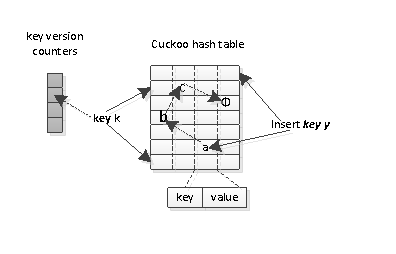
\includegraphics[width=0.9\textwidth]{cuckoo}
\caption{4路组相联Cuckoo哈希表}\label{fig:cuckoo}
\end{figure}

\subsection{Hopscotch哈希表}
与Cuckoo类似,Hopscotch也是采用的开放寻址法解决哈希冲突问题。
它在设计时综合考虑了Cuckoo哈希,线性探测法和链式法的特点,并将三者的优点结合起来。
Hopscotch哈希表由哈希桶数组构成。
它的核心概念在于任意的哈希表内的元素,它周围的所有哈希桶都称为其邻居哈希桶。
邻居哈希桶具有一个重要的特性:在邻居桶内查找元素所需的开销与在被映射的桶中查找元素所需的开销相同或者非常接近。
这个特性专门为处理插入操作而设计的。

图\ref{fig:hopscotch}实例描述Hopscotch插入元素的过程。
元素被映射进的实体总是在经过哈希函数计算得到的实体内或者在其相邻的下一个H-1实体内,其中H是设定的常量(一般H为32或者64位,一个标准机器字长),可以根据需求进行调整。
每一个实体包含一个字节的’跳‘信息和一张H比特的位图,位图指示在当前实体的下H-1个实体内包含该元素的虚拟桶的偏移量。
通过查看‘跳’信息能够得知哪些实体属于同一个哈希桶,然后只需扫描常数级别的实体数量快速的找到某一元素。
从任意相邻桶内找出某一特定元素的开销等同或者非常接近于直接从该元素所属的桶内进行查找的开销。


总之,Hopscotch的设计思想就是将空闲的槽位向着目标哈希桶移动,或者像Cuckoo哈希那样将元素从目标桶中移除然后重新为其寻找合适的位置。
Hopscotch实现了串行和并发两个版本~\cite{hopscotch},本文中用到的支持多线程并发的Hopscotch。

%cuckoo数据结构
\begin{figure}[htbp]
\centering
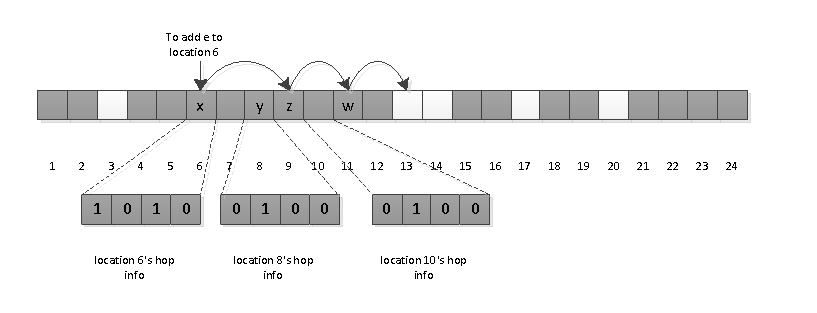
\includegraphics[width=0.9\textwidth]{hopscotch}
\caption{Hopscotch插入操作示例}
\label{fig:hopscotch}
\end{figure}

\subsection{基于RCU机制的哈希表}

\textcolor{red}{spilted-order list有基于URCU的实现版本,具体参看谷歌搜索urcu hash table的结果。}

读-复制更新,Read-copy Update(RCU)并不单纯是一种并发哈希表的设计方案,它最初是一种用于优化Linux系统内核的共享数据访问的一种并发模型~\cite{rcu}。
RCU是一种无锁化编程模型。
对于被RCU机制保护的共享数据结构,读者线程可以不需要锁自由的对其进行访问,但是写者线程在对该共享数据结构进行修改前必须保留该数据结构的副本。
当修改完成之后,通过适当的回调函数将指向旧数据的指针修改成指向新的数据(从旧数据拷贝的数据)。
RCU的核心概念有两个:一个成为静默期(quiescent state);一个称为优雅期(grace period).
\textcolor{red}{补充静默期和优雅期的描述与功能。}

基于RCU的并发哈希表的最大特点是牺牲更新性能来换取读性能。
基于RCU的编程模型主要用于Linux系统内核,为了便于将RCU集成到我们的测试框架下进行测试我们使用用户态的RCU实现(URCU)~\cite{urcu}~。
本文使用的URCU v-0.8.8版本~\cite{urcucode}。

\subsection{基于线程构建模块的哈希表}

Intel推出的线程构建模块(Threading Building Blocks, TBB)是一种针对多核平台的基于任务的并行编程模型~\cite{tbb}。
它实现的concurrent\_hash\_map允许多个线程并发的访问。
concurrent\_hash\_map的键是无序的。
每一个键在哈希表内最多只有一个元素与之相对应,但不排除有其它的元素尝试插入到相同位置。
类\textit{const\_accessor}和\textit{accessor}统称为访问控制器(accessor)。
访问控制器允许多个线程并发的访问哈希表内的键/值对。
访问控制器充当指向键/值对的智能指针。
它持有作用于键/值对上的隐式锁,直到该实例被销毁或者访问控制器调用解锁函数才会释放。

TBB实现的并发哈希表处理冲突采用的是典型的链式法。
键被哈希到包含了实体形成的链表的哈希桶内。
基于TBB的并发哈希表继承了链式法的所有优缺点。
适合处理读占多数的数据集。
本文中,将TBB v 4.2集成到CHTBench中进行测试。

\section{并发哈希表的评估与分析}
\textbf{并发哈希表}(CHT)是一种允许在同一时刻有多个读者或写者访问共享对象的哈希表。
其提供与串行哈希表一样的访问接口,但是CHT能够更有效的发挥多核处理器的性能。
并发哈希表的性能不仅依赖于应用本身的需求而且还依赖于底层硬件特性。
所以,对并发哈希表的剖析不能单纯的停留在吞吐量、延迟等直观的指标上,而是要综合考虑微观和宏观,底层和上层等多个层面的影响。
进一步说,选用通用的测试评估指标在一个统一的测试框架下进行测试,处理不同的工作集时没有任何一种并发哈希表能全面的体现其优势。
另一方面,对于用户而言,能够预先知道某种CHT的性能障碍将对其挑选合适的并发哈希表提供帮助。
不幸的是,这种用户关切的问题在现有研究中鲜有人提及。
由于缺乏一个统一的测试框架,用户也很难通过自行测试进行比较而选出理想的CHT应用到其软件系统中。
总之,对并发哈希表进行全面深入的剖析对并发哈希表的使用、设计以及优化都具有深远意义。
基于以上考虑,我们从现有的并发哈希表中挑选出表~\ref{tab:concurrent_hash}中列举的五种比较突出的进行深入的分析。

具体的,将挑选的CHTs放入CHTBench的框架内进行测试,对并发哈希表的评估与分析将围绕并发哈希表的线程扩展性、更新比重对性能的影响、初始化的哈希表元素的规模对性能的影响、延迟、线程绑定方案、同步机制以及内存消耗等七个方面展开。

\subsection{测试平台与配置}
为了体现对并发哈希表的评估具有一般性,测试在4台基于不同体系架构的多核处理器上展开。
它们分别是AMD Opteron 6172,Intel Xeon E5-2630,Xeon E7-4850,以及Intel Xeon Phi 7120p。
表~\ref{tab:arch_info}~给出了4个平台的硬件和系统特征。
测试过程中为了避免因操作系统的差异引入的干扰因素,所有测试平台都搭载Ubuntu 14.04 LTS操作系统。
下面分别对4台机器的硬件特征逐一进行介绍。

%目标平台的硬件和系统特征
\begin{table}[htbp]
  \centering
  \caption{测试目标平台的硬件和系统特征}
  \label{tab:arch_info}
  \begin{tabular}{ccccc}
    \toprule
       名称             & AMD Opteron           & Intel E5-2630       & Intel E5-4850     & Intel MIC \\
    \midrule
      系统               & Magny Cours      &  Ivy Bridge-EP        &  Haswell-EX         &  Knights Coner \\
      处理器             &  Opteron 6172         &  Xeon E5-2630      & Xeon E7-4850     &  Phi 7120P \\
      核/线程数量         & 24/48                & 16/32                & 48/96              & 61/244 \\
      时钟频率(GHz)       & 2.1                  & 2.4                  & 2.3               & 1.238 \\
      L1缓存(KB)         & 64/64 I/D             & 32/32 I/D            & 32/32 I/D         & 32/32 I/D \\
      L2缓存(KB)         & 512                  & 256                   & 256               & 512 \\
      LLC缓存(MB)        & 2x6                  & 20                    & 24                & NULL \\
      互联通道            & 6.4 GT/s HT          & 2x QPI               & 3x QPI             & NULL \\
      最大内存带宽(GB/s)   & 42.7                 & 51.2                 & 68                & 352   \\
      % 内存型号            &                       &                     &                   &         \\
      主存(GiB)         & 128                   & 56                  & 128                & 16 \\
    \bottomrule
  \end{tabular}
\end{table}

\begin{figure}[htbp]
\centering
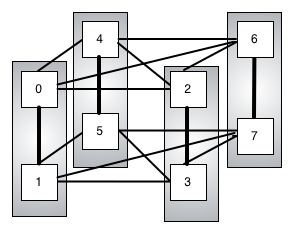
\includegraphics[width=0.6\textwidth]{AMD_top}
\caption{AMD Opteron内存结点拓扑结构}\label{fig:AMD_top}
\end{figure}

\textbf{AMD Opteron.} 该48核的AMD Opteron机器包含4个Opteron多芯片模块(MCMs)。
该系统总共具有八个内存结点:每一个MCM分为2个片区,每个片区拥有6个核,各个片区使用独立的内存控制器进行控制。该系统的拓扑结构如图~\ref{fig:AMD_top}~所示。
位于同一个多芯片模块内的两个片区之间的距离定义为1跳(1-hop),位于不同多芯片模块上的两个片区距离为2跳(2-hop)。
多芯片模块内通信开销要低于多芯片模块间的通信开销,并且模块内的两个片区之间的共享带宽比位于两个不同模块内的片区间的共享带宽要高。
它的CPU的时钟频率为2.1 GHz,三级缓存的容量分别为64 KiB,512 KiB和4 MiB (每一个片区的私有缓存容量)。
总的运行内存为128 GiB。
Opteron的缓存具有回写和非包容性~\cite{Conway2010Cache}。
然而,存储的层次结构并不具备严格的排他性,也就是说在LLC中命中的数据会被推送到L1中,至于该数据会不会在LLC中被删除取决于硬件实现~\cite{2011Software}.
Opteron采用MESI的扩展性协议MOESI作为缓存一致性协议。
其中’O’表示占有(Owned)状态,它表示缓存行的内容被修改,与内存中的数据不一致,不过在其他的核上可能有这份数据的副本。

\textbf{Intel Xeon E5-2630.} Intel Xeon E5-2630由两路插槽组成,每路插槽中有8个物理核(16个硬件线程),它的运行内存为16 GiB。
它的时钟频率为2.4 GHz,三级缓存的容量为别为32 KiB,256 KiB 和20 MiB。
该系统具有4个内存通道和两条6.4 GT/s的快速互联通道(QuickPath Interconnect, QPI)。
E5-2630的最大内存带宽可达59 GB每秒。
它的缓存具有包容性,即就是说每一个新的缓存行的填充都将在三级缓存中同步~\cite{intel2016}。
最后一级缓存是回写的,当出现由空间不足或者一致性问题引起处于‘M’状态的缓存行被驱逐时,数据被写入到内存中。

\textbf{Intel Xeon E7-4850.} 该平台由4个插槽组成,每个插槽内有12个物理核(24硬件线程),它的运行内存为128 GB,时钟频率为2.3 GHz。
它的三级缓存的容量分别为32 KB,256 KB和24 MB。
它具有4个内存通道和3个QPI。
该机器的最大内存带宽为68 GB每秒。
它采用的缓存一致性协议与E5-2630相同.

\textbf{Intel Xeon Phi 7120p.} 该机器在同一片芯片上集成了64个有序内核。
每一个内核均支持最多四个硬件线程,因此该机器的最大硬件线程数量可达244个之多,单个内核的时钟频率为1.23 GHz。
Intel Xeon Phi 7120p的内存分层结构类似于传统的多核系统。图~\ref{fig:phi_arch}~所示为其体系结构.
Phi上的内存为所有核所共享,所有的内核均可对其进行访问,该机器的内存大小为16GB。每一个核都有一个大小为32KB的一级数据缓存和32KB的一级指令缓存,以及一个大小为512KB的二级私有缓存,片上二级缓存的总量为31MB。
Phi实现了一个扩展的MESI协议,该协议的新颖性在于其将Shared状态扩展为一个基于目录的缓存一致性协议,这个协议简称为GOLS(Globally, Owned, Locally Shared),该协议的好处是能够共享被修改的缓存行,并且避免地址总线上的广播风暴。
每一次的缓存都通过查看GOLS协议来确定缓存行的状态。Phi的全局一致性的维护是通过纪录有每一个缓存行一致性状态的分布式目录标签(Distributed Tag Directories, DTDs)完成的。每一个缓存行的地址都通过一个哈希函数映射到DTD上,这样做的好处是保证负载均匀分布。

\subsection{线程扩展性}

线程扩展性是指在多核平台上随着被创建的线程数量的增加,应用的吞吐量保持不减的趋势。
线程扩展性直观的体现在吞吐量上,吞吐量也是很常用的性能评价指标之一。
吞吐量的计算方式用执行的哈希表查询、插入和删除操作的总和除以执行完成这些操作所耗费的时间。
单位用百万操作每秒(Mops/s)表示。

\label{sec:thread_scal}
\subsubsection{总体的扩展性评估}

本次实验中,采用紧凑的线程绑定方案(具体见~\ref{sec:thread_pinning}~),每次测试的持续时间为5秒,实验的结果如图~\ref{fig:thread_scal}~所示,每一组参数配置都运行五次,最终结果取五次结果的平均值。

从图~\ref{fig:thread_scal}~的曲线变化可以观察到,在这样的参数配置下,URCU在多个平台上的吞吐量曲线几乎与x轴重合,也就是说在更新比重为10\%的情况下,URCU的性能很糟糕。
而CLHT(由于CLHT-lb和CLHT-lf之间的趋势相同,数值接近,故不单独进行讨论)则在4个平台上均展现出最佳的性能,这得益于它的设计出发点:尽可能的减少缓存行的切换次数。
Hopscotch的吞吐量在E5-2630和E7-4850两台机器上达到峰值时对应的线程数分别为16和24.值得注意的是,16和24正是这两台机器单个内存结点(socket)支持的最大线程的数量。
同样的它在AMD Opteron上的峰值出现在线程数为6这个点(6恰好是该机器同一片区支持的最大线程数)。
综合Hopscotch在三个NUMA架构平台上的表现,可以推断Hopscotch在降低跨内存结点通信开销方面存在缺陷,它在单内存结点的多核计算机平台上应该有不错的线程扩展性。
换句话说就是Hopscotch在利用NUMA系统特性上所做的优化粒度不够,更多的细节描述见~\ref{sec:thread_pinning}~节。

%Intel Phi 7120p 体系结构
\begin{figure}[htbp]
\centering
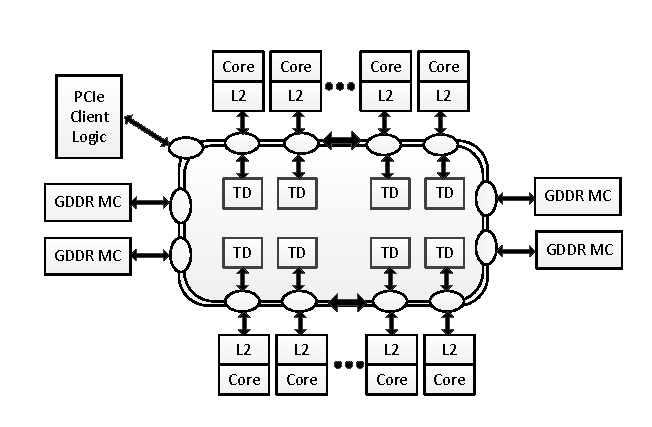
\includegraphics[width=0.9\textwidth]{PHIarch}
\caption{Intel Phi 7120p体系结构}\label{fig:phi_arch}
\end{figure}

考虑到在图~\ref{fig:thread_scal}~(a)中当线程数为16时存在一处拐点,故将该平台上的性能曲线单独分成两个阶段进行说明。

\textbf{阶段1}:在这个阶段创建的线程数量在1到16这个范围内,超线程没有被启用(紧凑型线程绑定方案)。
很明显CLHT表现出最佳的吞吐量增长速率,每多创建一个线程,它的吞吐量大约增加15 Mops/s。
CLHT-lb的性能优于CLHT-lf版本。对Hopscotch而言,每多创建一个线程,吞吐量大约增加5.5Mops/s. 在该阶段Cuckoo的性能比TBB要差。

\textbf{阶段2}:在这个阶段,创建的线程数量大于16个,线程分布在两个不同的插槽内而且超线程在这个阶段也被启用参与运算。
可能受到内存带宽上限的影响,CLHT的吞吐量保持微弱的增长势头。表~\ref{tab:mem_bandwidth}~列出了在Intel Xeon E5-2630平台上CLHT-lb的内存带宽随着线程数量的变化情况。
该表中数据表明在该阶段CLHT-lb运行时内存带宽没有发生变化。
而Hopscotch性能的陡然下降揭示它在处理跨插槽通信上的性能开销远大于增加额外的线程带来的性能增益。在这个阶段Cuckoo和TBB展现出不错的增长速度。

%表2,内存带宽使用情况
\begin{table}[htbp]
  \centering
  \caption{CLHT-lb内存带宽随线程数量变化情况}
  \label{tab:mem_bandwidth}
  \begin{tabular}{cccccccccc}
    \toprule
       Threads & 1 & 4 & 8 & 12 & 16 & 20 & 24 & 28 & 32 \\
    \midrule
      内存带宽(单位:GB/s) & 1.5 & 5.8 & 11.2 & 12.8 & 12.8 & 12.8 & 12.8 & 12.8 & 12.8 \\ 
    \bottomrule
  \end{tabular}
\end{table}


\begin{figure}[htbp]
\centering
%\subfigure[Intel]{
\subfigure[E5-2630]{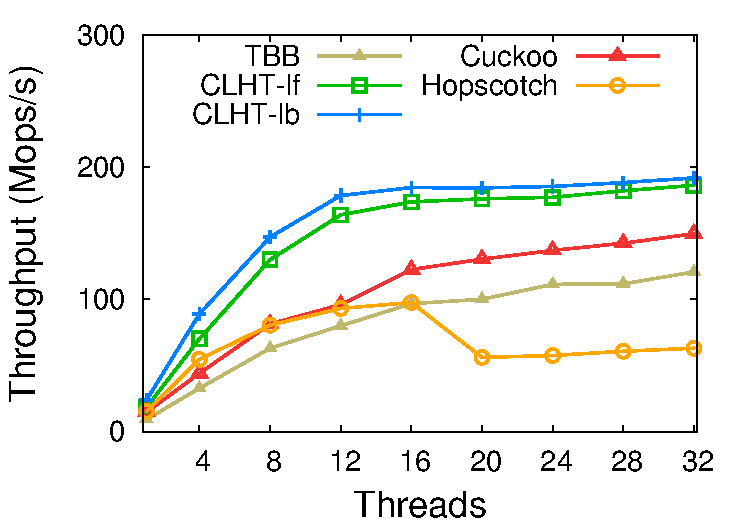
\includegraphics[width=0.45\textwidth]{2630Scal}}
\subfigure[E7-4850]{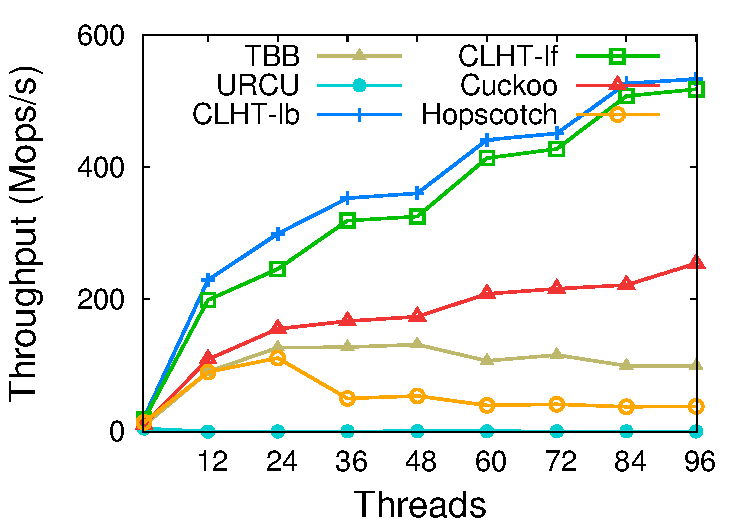
\includegraphics[width=0.45\textwidth]{4850Scal}}
\subfigure[Opteron]{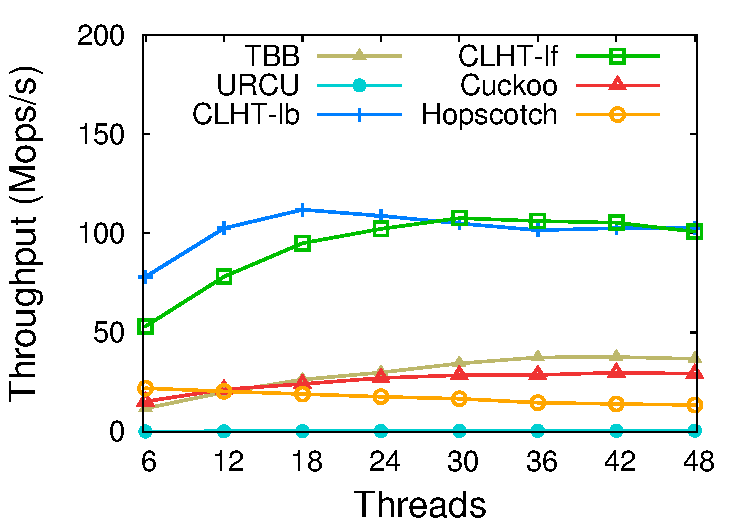
\includegraphics[width=0.45\textwidth]{AMDScal}}
\subfigure[Phi 7120P]{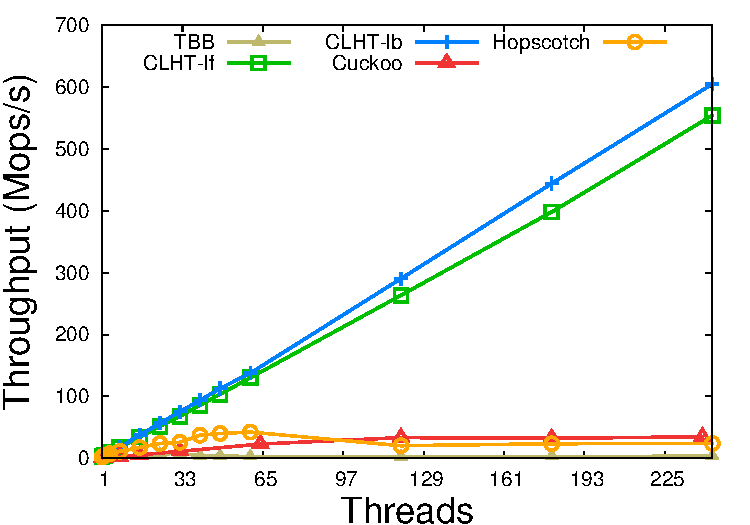
\includegraphics[width=0.45\textwidth]{7120PScal}}
\caption{并发哈希表的吞吐量随线程数量的变化曲线,哈希表的密度为50\%,\textit{u}为10\%,\textit{i}为一百万。}
\label{fig:thread_scal}
\end{figure}

图~\ref{fig:thread_scal}~(b)刻画的是E7-4850平台上的吞吐量曲线。
除CLHT之外,其它几种并发哈希表的性能曲线走势与E5-2630相似。
前面介绍了在E5-2630平台上由于受到内存带宽的限制,CLHT的吞吐量在第二阶段基本没有增长,而在E7-4850平台上CLHT全程保持稳定的增长趋势。

图~\ref{fig:thread_scal}~(c)给出的是AMD机器上的运行结果。
在该机器上TBB的线程扩展性在5个并发哈希表中仅次于CLHT。
Hopscotch只有当线程分布在同一个片区内时(n<=6)才具备最佳性能,创建更多的线程并不能促进整体性能的提升。
另外,对于Cuckoo和CLHT,当创建的线程数量超过某个特定的值时,会引起吞吐量的下降,这种引起吞吐量下降的原因来自两个方面:一是受到内存带宽的限制;一是来自有限的资源被多个线程激烈竞争。

Xeon Phi 7120P上的实验结果如图~\ref{fig:thread_scal}~(d)所示。
CLHT的两个版本在该平台上获得了线性的线程扩展性,每多创建一个线程,相应的吞吐量会增加大约2.5Mops/s. 
CLHT在该平台上获得线性扩展性归因于两个方面:
其一,每一个哈希桶的大小等于缓存行的大小,这样大大降低了缓存行切换的次数。
并且数据对齐有利于避免多线程伪共享问题,多线程伪共享是影响Xeon Phi性能的主要因素之一。
其二,CLHT采用细粒度锁在一定程度上抑制了线程间的竞争。
然而,并不是所有的并发哈希表在Phi 7120上都能表现的如CLHT一般呈现线性扩展性,相比于其它几个平台Cuckoo和TBB在该平台上的性能非常差,创建更多的线程也无法保证性能的提升。详细的原因将在~\ref{sec:impact_update}~和\ref{sec:sync}节中阐述。

\subsubsection{数据分布方式对线程扩展性的影响}
在前面的实验中,键值对是用随机方法产生的,服从均匀分布。
但是在实际的应用场景下,数据完美的均匀分布只存在理想状态中,某些数据出现的频度存在两极分化,因此,人们会更加关注不同的数据分布形式下各哈希表的性能表现。
在这一部分内容中,我们将对服从zipf分布的数据集进行测试。
在本次测试中,参数配置比如哈希表密度,更新比重以及哈希表的初始化元素个数均与线程扩展性一节的参数设置保持一致。
图~\ref{fig:zipf}为运行服从zipf分布数据集的性能曲线(在几个平台上的性能变化趋势相一致,故我们只给出了在E5-2630上的实验结果)。
与图~\ref{fig:thread_scal}(a)中的实验结果进行比较,Cuckoo,CLHT,Hopscotch以及TBB的吞吐量分别下降44\%,51\%,53\%和30\%。
性能下降的原因在于zipf分布使得数据访问更加倾向于频度较高的键值对,造成多数的操作集中访问少数频度较高的数据内容。
这加剧了多个线程访问相同键的竞争程度,对片上互联通道和同步造成压力从而引发更多的缓存一致性流量。

%数据服从zipf分布时,CLHT-lb的线程扩展性
\begin{figure}[htbp]
\centering
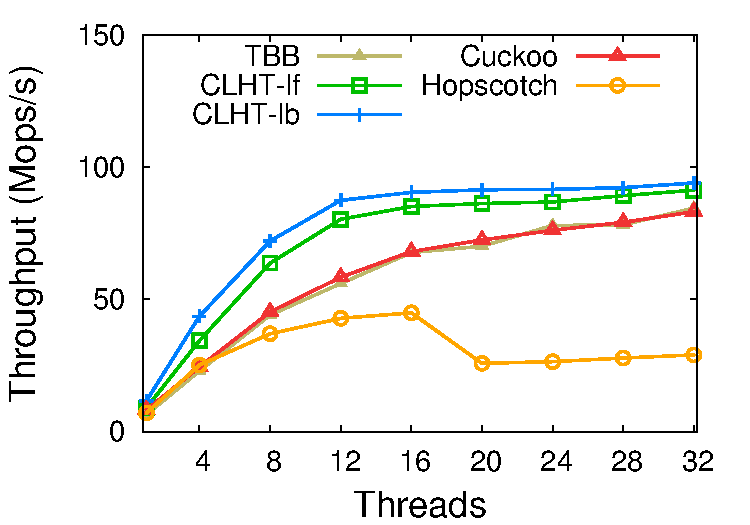
\includegraphics[width=0.6\textwidth]{2630zipf}
\caption{数据服从zipf分布时吞吐量随线程变化情况}
\label{fig:zipf}
\end{figure}

\subsubsection{哈希表的扩张}
不断的往哈希表中插入新的元素会引起哈希表密度的增加,将导致插入元素的时间成本增加。
在最坏的情况下,会因为找不到空闲位置并尝试多次之后导致插入操作失败,这无疑会对哈希表的性能造成巨大的损耗。
面对这样一种情形,大部分哈希表在设计的时候允许哈希表在达到一定密度后自行进行扩张。
具体的工作流程是,创建一张新的哈希表,新表的容量一般为旧表容量的两倍,然后将旧表中的元素拷贝到新表中,这不可避免的引入额外的时间和空间开销。
为了探究并发哈希表进行扩张时的开销情况,设计了如下一组实验。
在本次测试中,由于Hopscotch不支持哈希表的扩张,故没有比较,哈希表的初始化密度设为90\%,更新比重调整为40\%,其中插入占35\%,删除占5\%,这样设计的目的在于确保插入表中元素的个数大于被删除的元素个数,从而保证在运行过程中哈希表中元素的密度在不断的增加,增加触发哈希表扩张的概率。
实验结果表明,Cuckoo触发resize操作的概率低于TBB和CLHT,我们认为这得益于Cuckoo在查找cuckoo路径上所做的优化。在触发哈希表扩张操作的情况下,吞吐量大概下降5\%左右。

\textbf{分析}:创建更多的线程并不总是意味着吞吐量的增加。
一方面,创建更多的线程可能导致内存子系统达到饱和,从而导致性能不再上升甚至将削弱总体性能。
另一方面,NUMA系统在缺乏适当仲裁机制的情况下更高的并发度将引起高速互联通道的竞争居高不下,从而达不到最优性能。与传统的多核架构相比,Intel MIC架构在并发哈希的扩展性方面体现出重大差异。
在这种新的体系架构平台上设计并发哈希表需要充分考虑改种体系架构的特征。
处理倾向于高频度数据的访问的工作负载将引起更高的缓存一致性流量,这将需要更复杂的同步算法来缓解性能下降的问题。

\subsection{更新比重对性能的影响}
\label{sec:impact_update}
并发哈希表与串行哈希表一样善于处理读操作占多数的工作负载。
在本节中,通过调整工作负载中更新操作的比重来观察各个并发哈希表性能的变化情况。
哈希表中初始化元素的个数设置为一百万。
在三个NUMA架构平台上,选取\textit{n}为平台单个socket支持的最大线程数。
Phi 7120P上\textit{n}是选取一个能够展示线程扩展性的值。
这样,使用紧凑型线程绑定策略时可以避免跨socket流量的干扰。

\begin{figure}[htbp]
\centering
%\subfigure[Intel]{
\subfigure[E5-2630, n = 16]{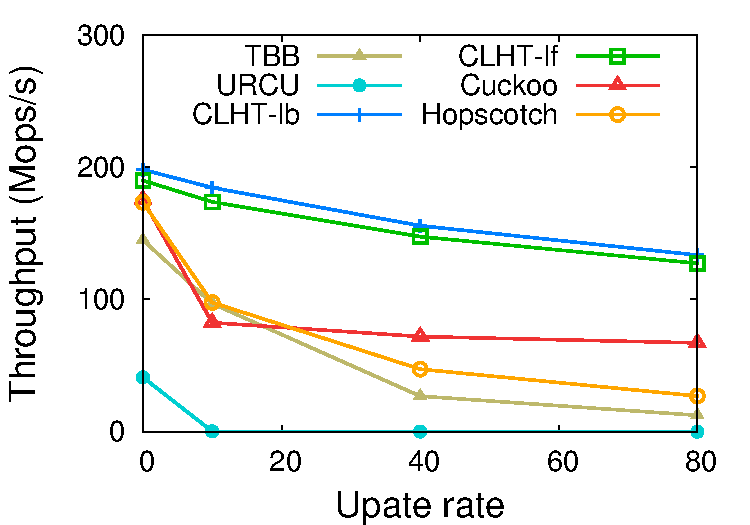
\includegraphics[width=0.45\textwidth]{2630Update}}
\subfigure[E7-4850, n = 24]{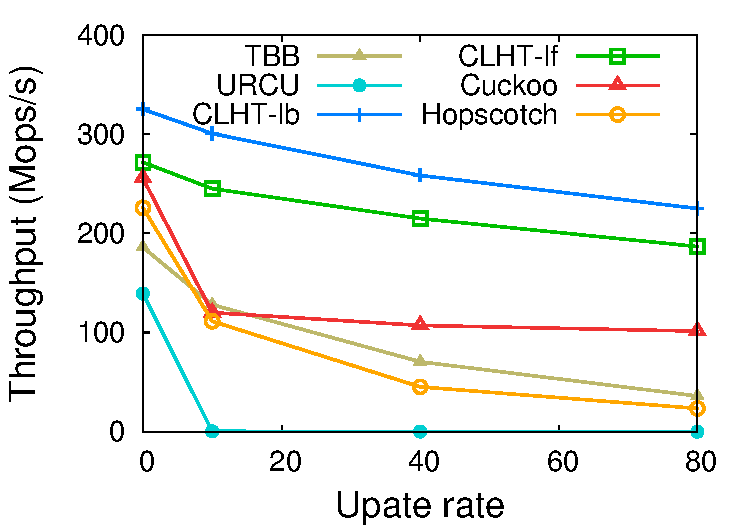
\includegraphics[width=0.45\textwidth]{4850Update}}
\subfigure[Opteron, n = 12]{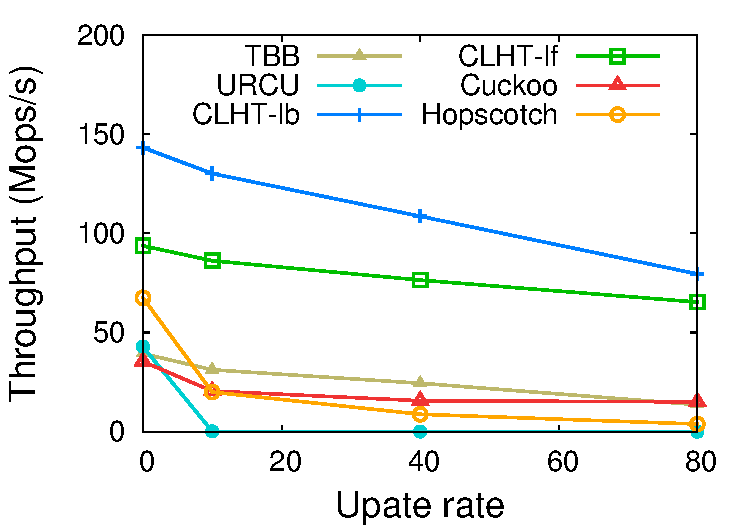
\includegraphics[width=0.45\textwidth]{AMDUpdate}}
\subfigure[Phi 7120P, n = 60]{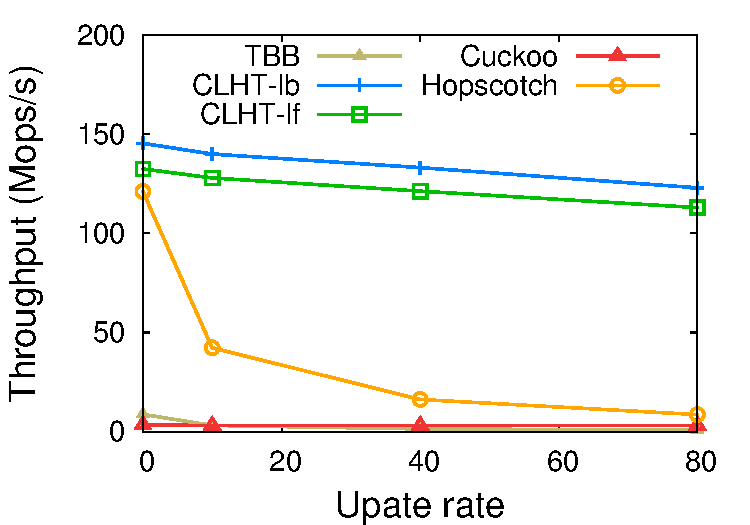
\includegraphics[width=0.45\textwidth]{7120U10}}
\caption{哈希表初始化元素个数一定的前提下,吞吐量随更新比重变化趋势}
\label{fig:update}
\end{figure}

如图~\ref{fig:update}~所示,
所有的并发哈希表的吞吐量峰值都出现在更新比重为0处,也就是说并发哈希表对处理纯读的工作负载具有最佳性能。
但是一旦运行的工作负载中包含了更新操作,性能会有很明显的下降。
其中URCU对于更新操作最敏感,更新比重从0调整到10\%,URCU的吞吐量下降到原来的1/270。下降幅度大的还有Hopscotch。
该现象同样解释了Hopscotch由于很高的同步开销导致的严重的扩展性问题(其它的并发哈希表比如TBB和URCU也有同样的问题)。
在更新比重增加时,Cuckoo表现出相对稳定的性能,它的下降速率在几个并发哈希表中是最低的,表明Cuckoo更能应对具有高更新比重的工作负载。

为了更好的说明工作负载中的更新比重发生变化引起性能变化的原因,本次实验引入一个新的微观指标:缓存未命中数/总的操作数量。
缓存未命中数用VTune Amplifier进行测量,测量结果为线程数16时的结果,具体见表~\ref{tab:cache_miss_update}。
通过表3的数据表明工作负载中更新比重越高,每操作对应的缓存未命中数也越高。
CLHT在低更新比重和高更新比重下都表现良好,这从表3中也可以得到体现,CLHT对应的最大值与最小值之间的差距只有30\%。
而URCU对应的值从0到10\%这个阶段扩大了14倍,从0到80\%更是扩大了127倍之多。
糟糕的情况更不止如此,URCU的CPU利用率非常低,大约保持在3\%左右,而同等参数配置下其它并发哈希表的CPU利用率达到50\%。进一步探究发现,
创建更多的线程并不会引起缓存未命中数量的增加,这表明工作负载中更新比重的变化是引起吞吐量变化的主要原因。

%表3,调整更新比重时缓存未命中率的变化情况
\begin{table}[htbp]
  \centering
  \caption{平均缓存未命中数量随更新比重变化情况}
  \label{tab:cache_misses_update}
  \begin{tabular}{ccccccc}
    \toprule
       更新比重(\%) & TBB & URCU & CLHT-lf & CLHT-lb & Cuckoo & Hopscotch  \\
    \midrule
     0 & 28.6 & 85.2 & 23.6 & 31.7 & 33.5 & 22.9  \\
      10 & 46.3 & 1169.2 & 24.6 & 34.9 & 44.2 & 28.1 \\
      40 & 99.2 & 4046 & 27 & 37.3 & 57.2 & 62.7 \\
      80 & 159.1 & 10788 & 30.7 & 40.6 & 66.2 & 115.5  \\
    \bottomrule
  \end{tabular}
\end{table}

\textbf{分析}:频繁的缓存行切换是并发哈希表更新性能最大的敌人。
更新操作致使缓存行失效的原因来自于两方面:一方面是写入本地内存结点的流量;另一方面是被缓存一致性协议强制进行的跨socket消息以及通过片上高速互联通道如Intel QPI和AMD HyperTransport等传递的信息。
一些设计用于处理读为主的工作负载的并发哈希表,哪怕是工作负载中包含很小部分的更新操作,它的性能也会大打折扣。
写友好型并发哈希表通常会进行精心设计用以控制缓存内的关键数据,比如共享变量等。

\subsection{缓存与主存}
考虑到哈希表属于内存密集型应用,所以在这一部分我们探究内存分层结构对并发哈希表性能的影响。
图~\ref{fig:initial_size}中的柱状图表示吞吐量随着哈希表初始化元素个数的变化情况,不同的初始化值所需的内存对应相应平台的三级缓存容量与主存容量。

\begin{figure}[htbp]
\centering
%\subfigure[Intel]{
\subfigure[E5-2630]{\includegraphics[width=0.45\textwidth]{2630Init}}
\subfigure[E7-4850]{\includegraphics[width=0.45\textwidth]{4850Init}}
\subfigure[Opteron]{\includegraphics[width=0.45\textwidth]{AMDInit}}
\subfigure[Phi 7120P]{\includegraphics[width=0.45\textwidth]{7120PInit}}
\caption{不同初始化大小对应的吞吐量抽样直方图}
\label{fig:initial_size}
\end{figure}

由于Phi 7120P与其它三个平台在内存分层结构上存在差异,故单独列出讨论。
从图~\ref{fig:initial_size}~(a)-(c)中观察到,当工作集的规模小于缓存的容量时,吞吐量是随着初始化大小增加的。
我们通过likwid-perfctr这个工具对最后一级缓存与主存之间的带宽与流量进行监测确认了这一结果。
一旦工作集的规模超过最后一级缓存的容量,将有较大的性能损耗。
此外,CLHT由于其在缓存使用机制上的独特设计,它的工作集规模小于缓存容量时的性能要比其它方法更好。
通过本次实验,我们还观察到一个有意思的现象(图~\ref{fig:initial_size}中没有体现该现象),当被创建的线程个数增加时,在一级缓存中存在显著的数据竞争情况。
下面通过举例对此现象加以说明,当初始化元素个数为1000时,并发哈希的吞吐量随着线程数量的增加而降低。
这个现象的原因在于线程越多,不同线程同时访问相同的共享数据的概率越高,从而导致较高的同步开销。

Hopscotch在本次实验中属于例外情况,它的吞吐量几乎不随初始化元素个数的变化而变化。
进一步的探究发现在Hopscotch的实现中,哈希表的内存是通过预先开辟固定大小的内存空间建立的。
这种方法的好处是获得了性能的稳定,缺点是丧失灵活性,在处理较小规模的工作负载时对内存空间的浪费较严重。
对高并发度的应用而言,无论是基于锁还是无锁的并发哈希表的实现,都依赖于有效的内存管理机制。而这些内存管理机制通常是建立在第三方插件的基础之上,或者来自由系统提供的动态内存分配器。
需要说明的是,有些并发哈希表在试图运行更大的工作负载(初始化值大于1亿)时失败了。这也可能是由内存管理上的缺陷造成的。

前文中指出,Phi 7120P的内存分层结构于其它主流多核体系架构存在较大差异。
它只包含两级缓存,并且其核与内存控制器之间是通过双向环状总线进行连接的。图~\ref{fig:initial_size}~(d)为Phi 7120P上的实验结果,在该平台上CLHT的吞吐量随着初始化元素个数的增加而降低,而其它几种哈希表因为数值太小在图中无法明确的体现这一趋势,通过比较实验数据发现同样符合这个趋势。

除了图~\ref{fig:initial_size}~中展示的数据规模之外,还对运行超过GB级别的数据进行了测试。
性能曲线与初始化值为一百万时的同类测试类似,只是在吞吐量上要打折扣。

\textbf{分析}:缓存对加速不同体系架构的性能具有非常重要的作用。
对缓存采用细粒度的方法进行控制的目的在于获得可预测的结果,比如为常驻缓存的工作集进行线程调度有利于避免额外的同步开销。
静态内存分配的方式对于并发哈希这种内存密集型应用来说并不是最佳选择,而对超大规模数据集使用动态内存分配方式需要进一步的优化方案予以辅助。

\subsection{操作延迟}
\label{sec:latency}
前文从宏观的吞吐量出发对并发哈希表进行了评估,在这一节当中我们从微观的每个操作执行的运行时延迟的角度进行分析。
对于延迟敏感型应用而言,理解不同算法设计的延迟变化造成的影响至关重要。

本次实验中,更新比重设置为10\%,哈希表密度为0.5,哈希表的初始化元素个数为一百万。
通过实验收集哈希表操作所耗费的CPU时钟周期数进行统计。
我们对哈希表的操作进行如下定义:如果某个操作完成了对其预期目标对象的访问,我们称该次操作为一次成功的操作;否则我们称之为一次失败的操作.
根据如上定义,得到六种不同的操作类型,它们分别记做:get-suc, get-fail, put-suc, put-fail, rem-suc和rem-fail。所需的时钟周期数使用开源工具sspfd~\cite{sspfd}~收集,然后通过均匀抽样方法计算每种操作对应的平均延迟。

图~\ref{fig:latency}给出了我们在E5-2630平台上的实验结果。
随着所创建的线程数量的增加,资源的竞争(包括内存带宽,缓存以及内存控制器)和同步开销逐步增加,这些都将不可避免的导致延迟的增加。
通过比较发现,CLHT(两个版本)在大部分情况下的延迟都低于其它并发哈希方法,这归因于它在设计上严格遵循4条异步并发模式。
过多的缓存行切换需要更周密的缓存一致性协议予以支持,从而导致哈希表操作延迟的增加。在几种并发哈希表中,URCU的操作延迟最高,原因是URCU在设计上有一个称为“RCU优雅时间”的等待期。Hopscotch的延迟对跨插槽通信相当敏感(对应图中线程数量大于8时的曲线变化)。
并且在Hopscotch进行删除操作时它的时间戳会被修改,用以确保同一时刻对该内存地址的查询操作失效,这一点类似于CLHT的原子快照方法。
Hopscotch和CLHT的不同之处在于Hopscotch需要存储共享变量,这将引起额外的缓存一致性开销。
另外,因为Hopscotch的锁在一进入解析阶段就已经获得,所以Hopscotch的更新操作对应的解析阶段包含了等待过程。这些设计都违背了异步并发模式的第二条原则:“除非对数据结构进行清零操作,否则在更新操作的解析阶段不要执行任何存储操作,也不要有任何的等待过程或者重试操作。”在最坏的情况下,Hopscotch的延迟比URCU的延迟还要高(图~\ref{fig:latency}(c)和(d))。

\begin{figure}[htbp]
\centering
%\subfigure[Intel]{
\subfigure[get-fail]{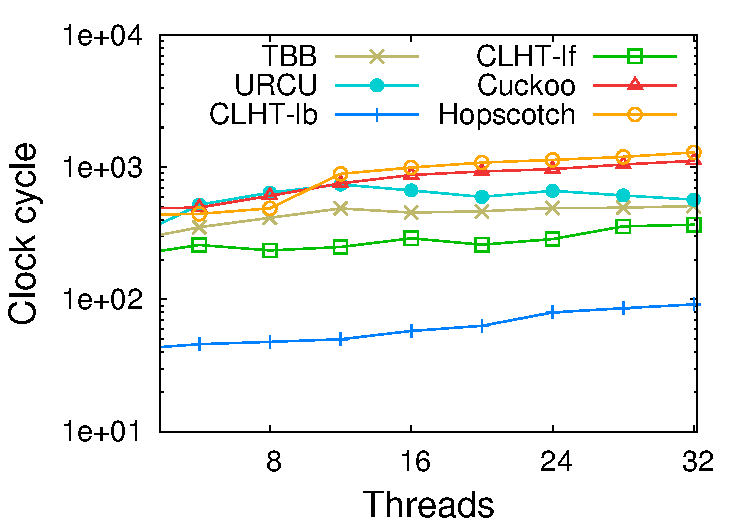
\includegraphics[width=0.45\textwidth]{getfail}}
\subfigure[get-suc]{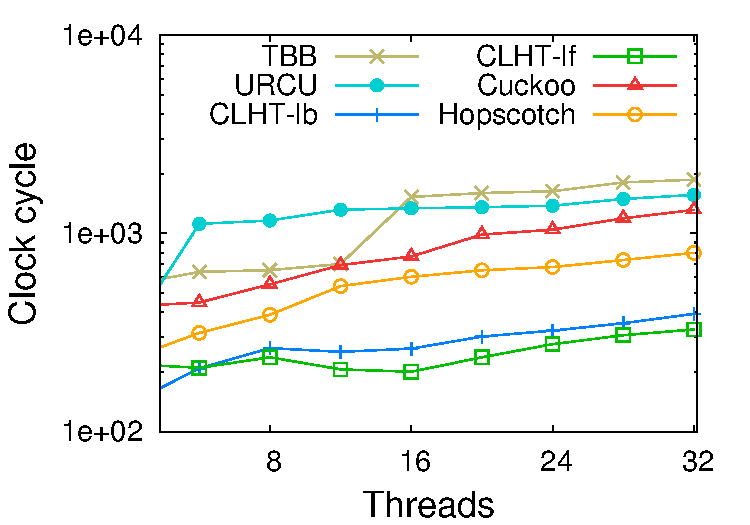
\includegraphics[width=0.45\textwidth]{getsuc}}
\subfigure[put-fail]{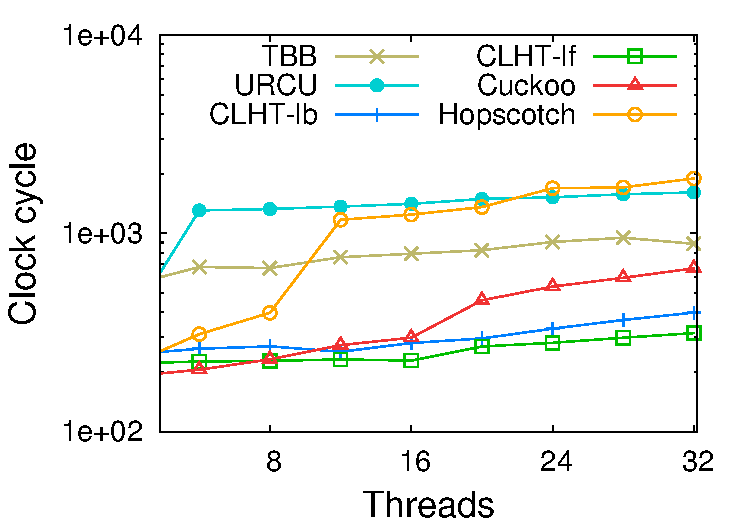
\includegraphics[width=0.45\textwidth]{putfail}}
\subfigure[put-suc]{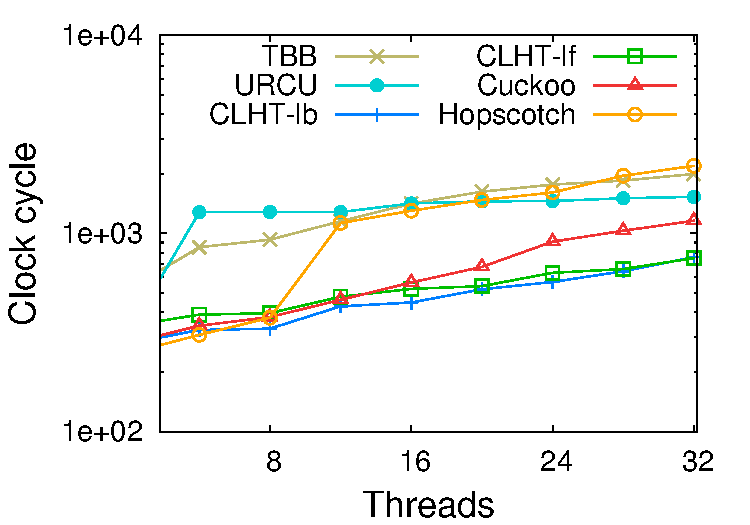
\includegraphics[width=0.45\textwidth]{putsuc}}
\subfigure[rem-fail]{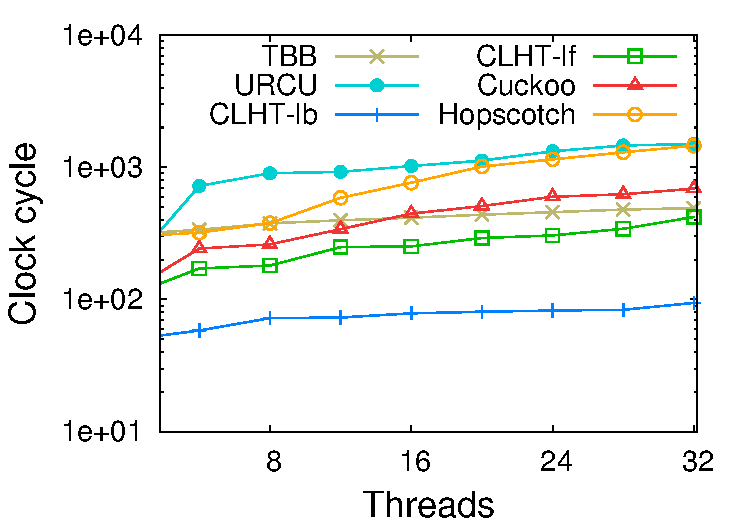
\includegraphics[width=0.45\textwidth]{remfail}}
\subfigure[rem-suc]{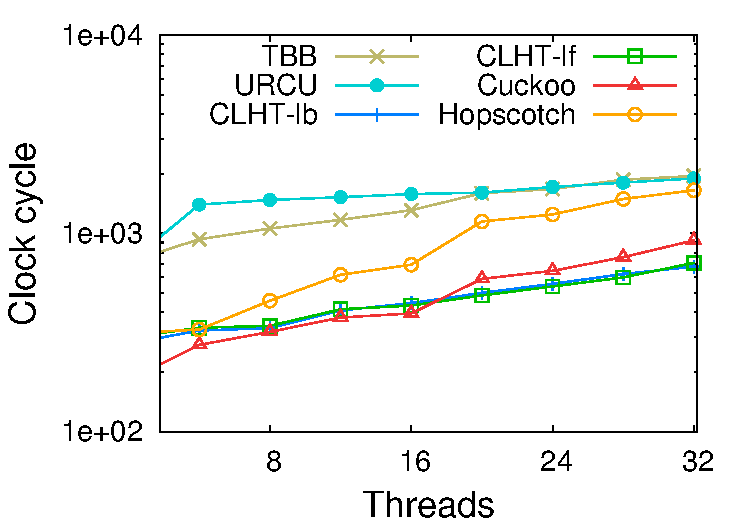
\includegraphics[width=0.45\textwidth]{remsuc}}
\caption{E5-2630平台上6种操作对应的延迟随线程数量变化曲线}
\label{fig:latency}
\end{figure}

Cuckoo从直观的计数器的数据来看它搜索操作耗费的平均时钟周期比更新操作的更高。
出现这种现象的原因是Cuckoo需要频繁的从较长的cuckoo路径中搜索元素。
在并发度较低的情况下,Cuckoo处理put-fail和rem-suc两种操作的延迟较低。
同样在线程数低于6的情况下,Hopscotch处理put-suc操作的延迟较低。TBB在处理fail类型的操作时的延迟相对稳定,但是在处理suc类型操作时与URCU持平,甚至在某些情况下比URCU表现更糟糕。

\textbf{分析:} David等人在其研究中提出的异步并发(ASCY)模式有助于获得良好的扩展性~\cite{clht}。
这一点在CLHT上得到很好的体现。
在实际应用中,ASCY的特定模式能够帮助开发人员在实现并发哈希表时避开潜在的陷阱。
比如,在对Hopscotch进行分析时,我们发现其在进行删除操作时对共享变量所做的修改,以及在更新操作的解析阶段的等待都与ASCY的原则相悖。
将删除操作替换成其它类型的操作进行测试发现其吞吐量有明显的增加。

\subsection{线程绑定方案的影响}
\label{sec:thread_pinning}
在多核计算机系统上线程到核之间的映射关系称为线程绑定。
线程绑定对于并发编程至关重要~\cite{pinning}。
在这一部分内容中,将以E5-2630为例,探究3种不同的线程绑定方案在4个多核系统上的表现有何区别。
图~\ref{fig:2630topology}所示为E5-2630平台上使用平衡型线程绑定方案时线程与核的映射拓扑结构。
该拓扑结构使用开源工具\textit{likwid}\cite{likwid}的\textit{likwid-topology}得到。
该平台具有两个socket,每个socket集成了八个物理核,每个物理核最多支持两个硬件线程。

\begin{figure}[htbp]
\centering
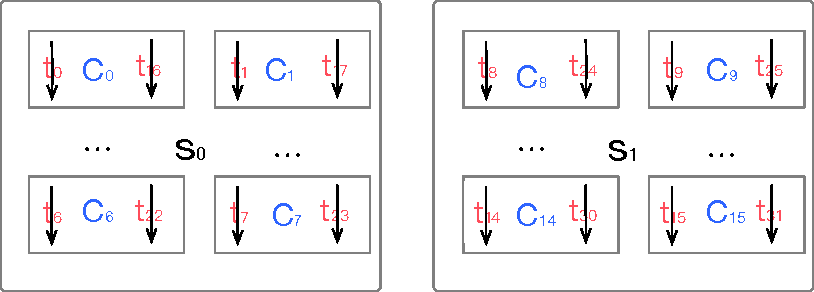
\includegraphics[width=0.6\textwidth]{2630topology}
\caption{E5-2630平台上使用平衡型线程绑定方案时线程与核的映射拓扑结构}
\label{fig:2630topology}
\end{figure}

在进行实验分析前,首先简要介绍实验中用到的三种不同方案:默认绑定方式和显示绑定方式,其中显示绑定方式又分为紧凑型绑定和平衡型绑定两种。

\textbf{默认方式}:线程通过系统调度器自动分配核。
操作系统调度器尽可能的实现多个核之间的负载均衡。这种绑定策略的好处是允许线程在执行过程中在不同的核之间迁移。

\textbf{紧凑型}:尽可能的将连续的线程映射到在拓扑结构上距离最近的核上。
如果需要创建24个线程,根据紧凑型绑定策略首先将第一个插槽内的核映射满,即就是线程t$_0$到t$_{15}$被映射到s$_0$内的c$_0$到c$_7$上,然后余下的线程将映射到位于s$_1$上的c$_8$到c$_{11}$上。
这种绑定方式的好处是在线程间提供较高的数据重用率。

\textbf{平衡型}:紧凑型线程绑定方案具有在单个插槽内共享缓存的优势,它的劣势在于紧凑型的线程绑定容易引起负载不均衡。
因此,平衡型绑定策略将线程均衡的绑定到位于不同socket的核上。
下面用一个实验测试中的实例进行说明:假设运行某次测试需要创建16个线程参与运算,正好可以将16个线程分别映射到c$_0$到c$_{15}$;
如果需要创建的线程数量超过了系统核的数量,这时才会启用超线程。使用平衡型绑定策略的好处有两方面:一是保持负载均衡;二是,在创建的线程数量少于系统具有的物理核的数量时,可以避免启用超线程产生的干扰。


\begin{figure}[htbp]
\centering
%\subfigure[Intel]{
\subfigure{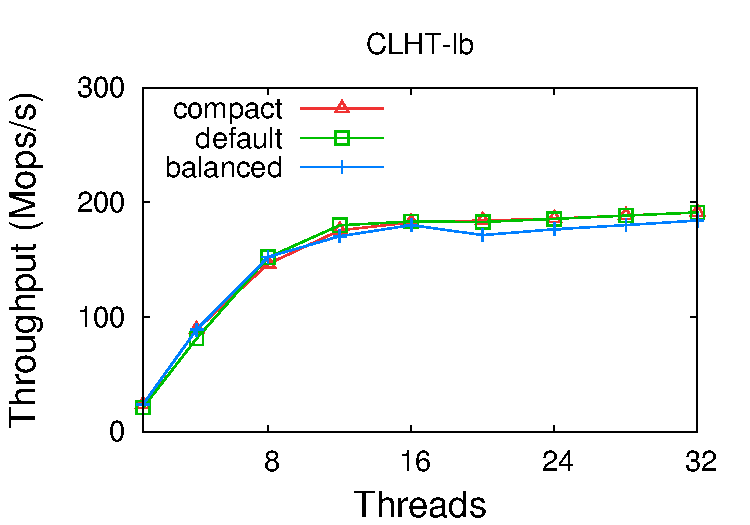
\includegraphics[width=0.3\textwidth]{2630clht}}
\subfigure{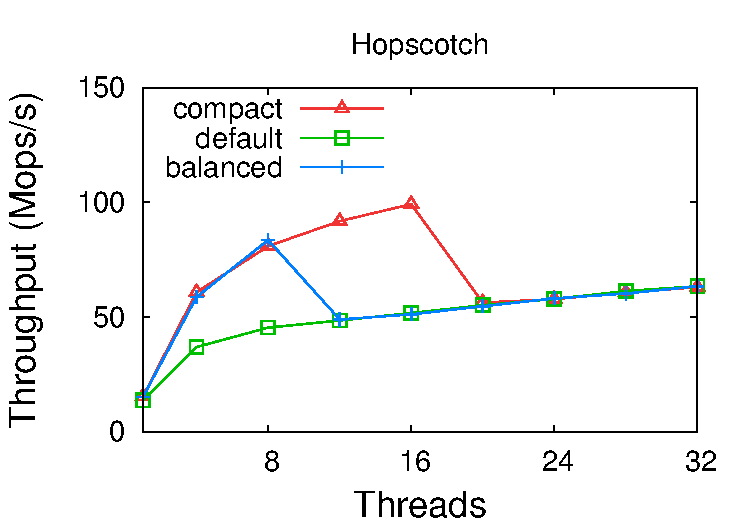
\includegraphics[width=0.3\textwidth]{2630hop}}
\subfigure{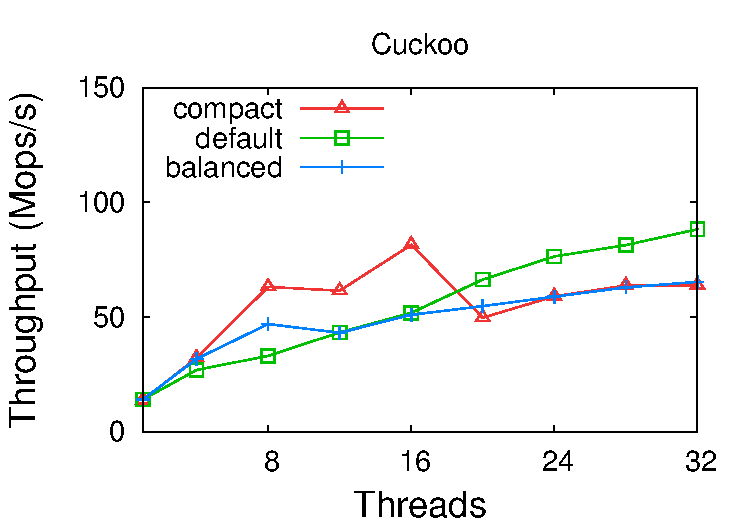
\includegraphics[width=0.3\textwidth]{2630cuckoo}}
\subfigure{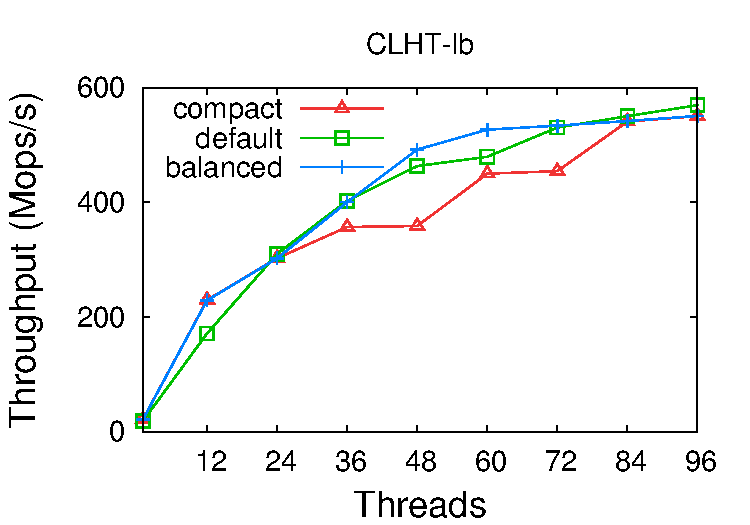
\includegraphics[width=0.3\textwidth]{4850clht}}
\subfigure{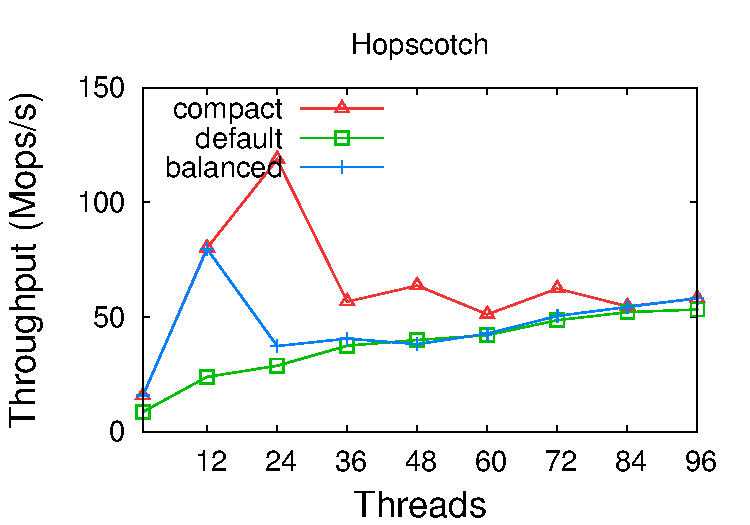
\includegraphics[width=0.3\textwidth]{4850hop}}
\subfigure{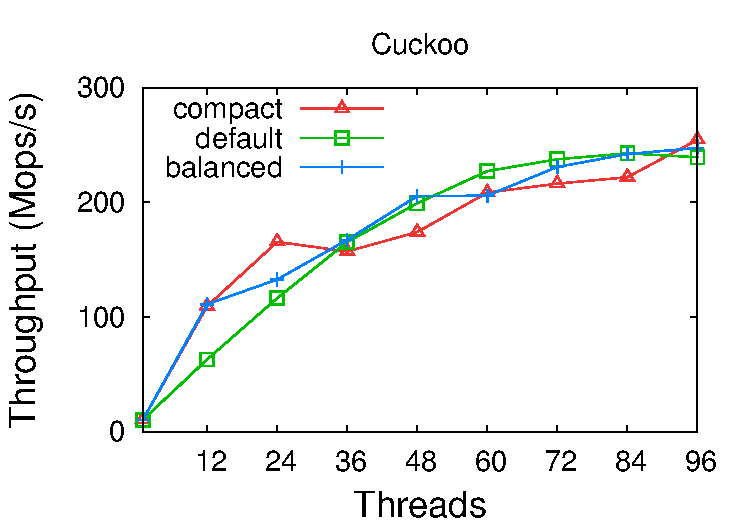
\includegraphics[width=0.3\textwidth]{4850cuckoo}}
\subfigure{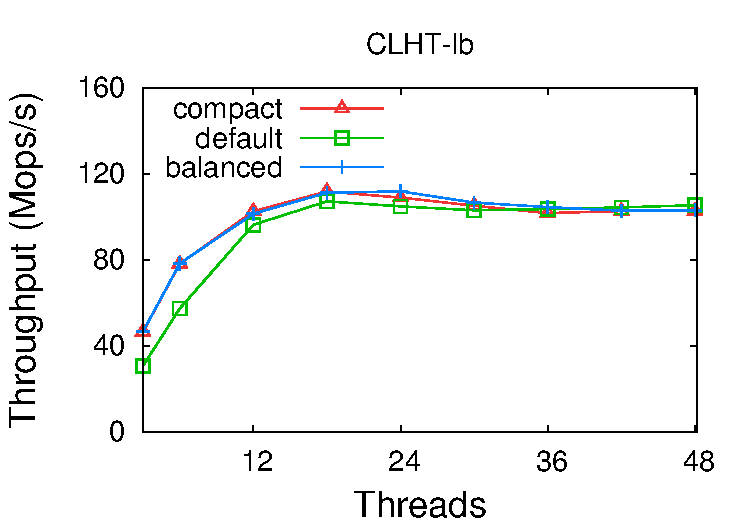
\includegraphics[width=0.3\textwidth]{AMDclht}}
\subfigure{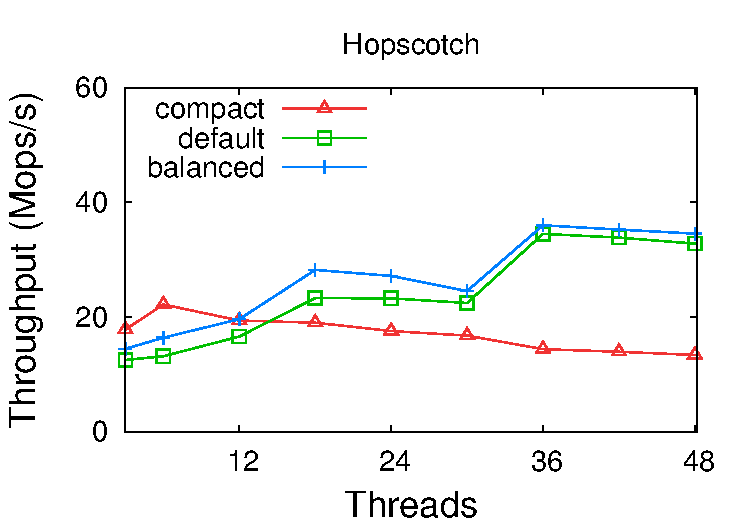
\includegraphics[width=0.3\textwidth]{AMDhop}}
\subfigure{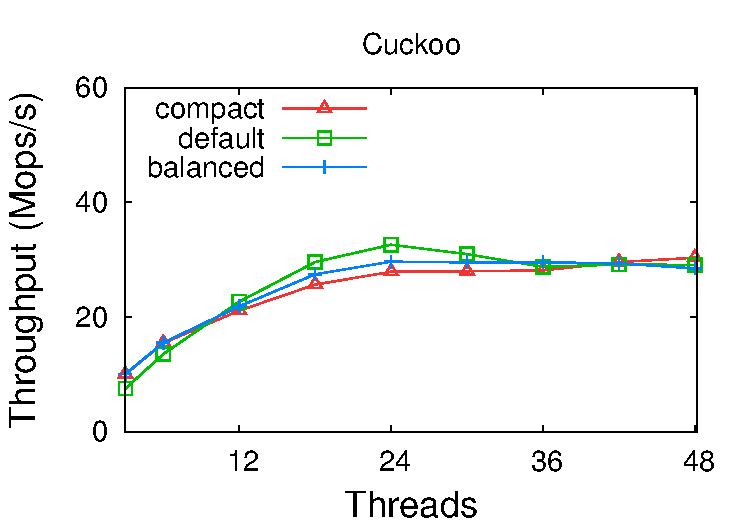
\includegraphics[width=0.3\textwidth]{AMDcuckoo}}
\subfigure{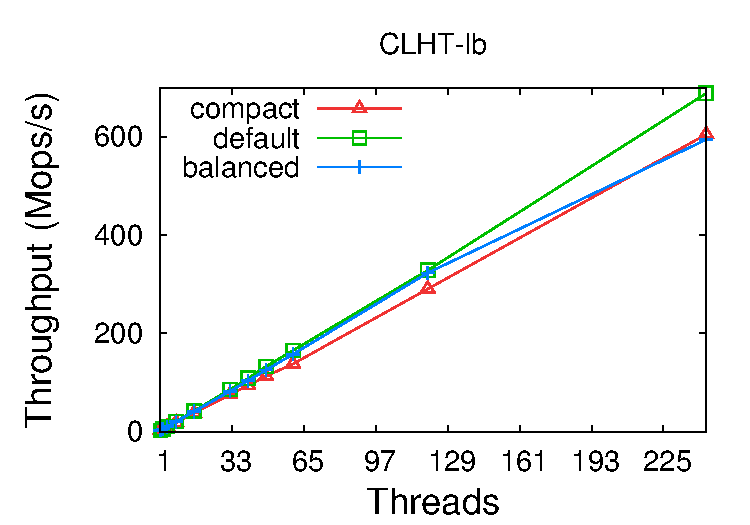
\includegraphics[width=0.3\textwidth]{7120Pclht}}
\subfigure{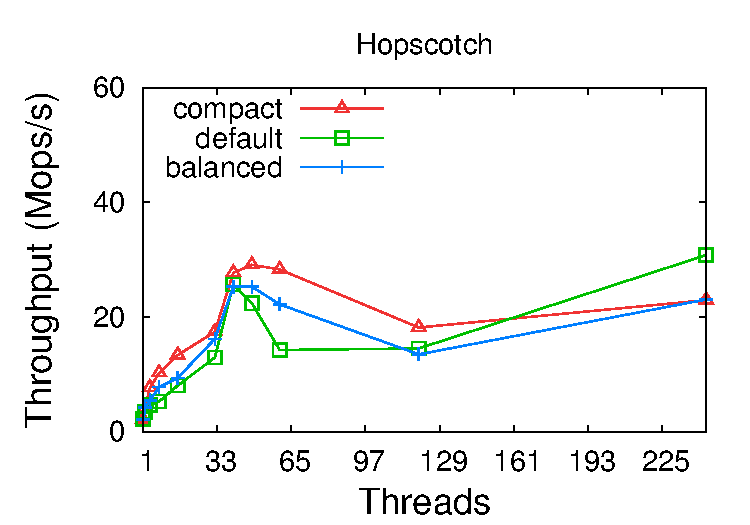
\includegraphics[width=0.3\textwidth]{7120Phop}}
\subfigure{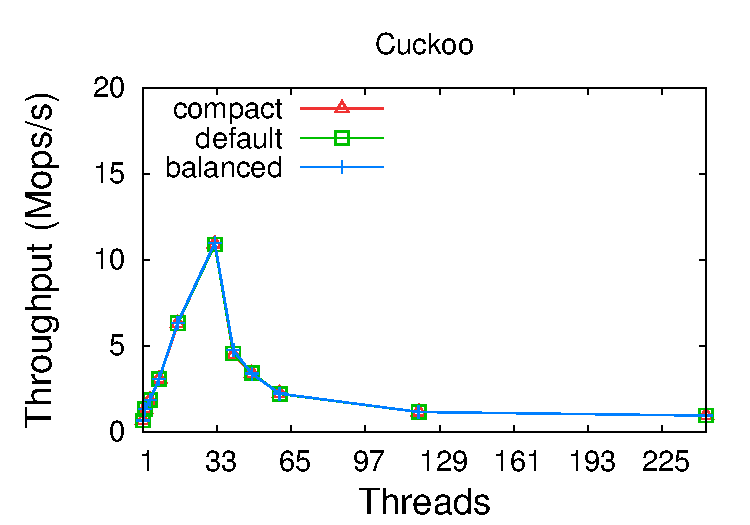
\includegraphics[width=0.3\textwidth]{7120Pcuckoo}}
\caption{三种线程绑定方式性能对比}
\label{fig:pin}
\end{figure}

CLHT的吞吐量受线程绑定方式影响较小,但Hopscotch和Cuckoo的吞吐量的波动却很大。
具体的以E5-2630为例,在该平台上以默认方式的性能曲线为基准,线程数量为8时,使用紧凑型和平衡型绑定策略性能提升了大约一倍。
进一步分析,在紧凑型线程绑定策略下,线程数达到16时,吞吐量比采用默认绑定方式提升了2倍。在E7-4850机器上体现了相同的趋势,故不再单独分析。

Hopscotch吞吐量显著的加速比来自于它的静态内存分配机制。
它在创建哈希表的同时就已经预先进行了内存分配,受Linux内核first 
touch内存分配策略的控制,预先分配的后果是导致所分配到的内存全部位于同一个NUMA结点上。所以,我们使用libnuma对其它并发哈希表进行优化,使其在进行动态内存分配时均衡的兼顾所有NUMA架构下的内存结点。
然而,当线程数从16向20变化(E5-2630),从24向36变化(E7-4850)过程中,吞吐量猛然下跌,这说明跨socket开销对性能的影响远大于此阶段参与运算的线程数量的增加。

而在AMD平台上,各哈希表的性能表现得对于线程绑定方式不敏感,这个现象可以从两个方面进行解释。
首先,Intel Xeon最后一级缓存的可包容性提供了较强的局部性,这种局部性提高了socket内通信的效率。
其次,在执行状态为’O’和’S’的缓存行上执行存储操作时,即便是所有的共享线程全部位于同一个socket内,AMD Opteron的不完整目录协议也会是跨socket间的流量失效。
因此,socket内的性能与跨socket情况下的性能基本一致。
由于负载的均衡分布使得该平台对跨socket通信不敏感,所以当线程分布在多个socket上时,默认绑定方法和平衡型绑定方法的性能要优于紧凑型绑定方式。

在Phi 7120P平台上,CLHT无论采用哪种绑定方式,性能都一如既往的好(吞吐量随着所创线程数量的增加呈线性增长)。
而Cuckoo采用三种不同绑定方式所获得的吞吐量不存在显著差别(三条性能曲线基本重合)。
这一点与之前在其它三个NUMA平台上观察到的结果存在较大差别,在NUMA平台上Cuckoo采用默认绑定方式具有最佳性能。
当线程数在[1,150]这个区间变动时,Hopscotch在Phi平台上使用紧凑型绑定策略获得最佳性能。
然而,在线程数超过150个之后,CLHT 和Hopscotch在这个阶段使用默认绑定策略的性能要优于其它两种策略。使用显示线程绑定策略的缺点是:受到二级缓存容量的限制,会造成更多的缓存未命中数量和过高的内存访问延迟。而在Xeon Phi上,默认绑定方式由于依赖于操作系统的调度器进行线程绑定并且允许线程在不同的核之间进行动态迁移,能够有效的降低资源竞争率并且更好的利用缓存子系统。
另外,Xeon Phi的表现类似与对成多处理机(SMP)系统,所有核到主存储器之间的距离是相等的。
将线程分配在不同的物理核上引起的开销与类似于NUMA系统上跨插槽的开销,但由于Phi上快速双向环状互联通道的设计使得跨核开销要远小于跨插槽开销。

\textbf{分析:} 通过实验表明没有哪一种绑定策略能在所测试的多个硬件平台上具有压倒性优势,也没有哪一种策略能够让所有的并发哈希表发挥最佳性能,所以在比较三种不同的线程绑定方案过程中没有一个统一的结论。
比如,在Intel Phi平台上,CLHT使用默认绑定方式具有最佳性能,但是在其它平台上则是其它绑定方式下具有最佳性能。
再就是Cuckoo在Phi平台上使用三种不同绑定方案的性能相当接近,没有哪一种具有明显的优势。因此,要探究并发哈希表的异常表现,需要结合并发哈希表的设计模式,线程绑定方案,创建的线程数量以及对应的硬件平台的特征进行考虑。
这对开发人员无疑是一种负担,最理想的解决方案是在运行过程中通过对硬件特征和工作负载的监控进行自适应的动态切换线程绑定策略,以达到获得最佳性能的目的。

\subsection{同步}
\label{sec:sync}
在并发读写的过程中,为了保障性能,多个线程对共享数据的访问需要用到同步方案对并发线程进行协调。
因此,设计并发哈希表时的另一个重要环节是同步方式的选取。
对线程间的同步处理不当会成为阻碍相关算法扩展性的最大障碍。
在这一部分中,将讨论并发哈希表中几种主要的同步机制以及运用不同的同步机制对性能会产生什么样的影响。

回顾图~\ref{fig:update}的性能曲线,几种并发哈希表中CLHT的性能最突出,尤其是在Phi 7120P平台上体现的最为明显。
CLHT获得突出线程扩展性的原因除了其在数据结构设计上的巧妙之处外,它所采用的同步机制的贡献也不容忽视。CLHT-lb使用原子快照对读者线程和写者线程进行同步。
具体的,在读者线程间,它使用由原子操作FAI(Fetch-and-Increment)实现的自旋锁对每个哈希桶进行保护。
采用这种方式的好处是,即便在并发度很高的情况下,竞争仍然保持一个较低的水平。
简单锁方法加上低竞争化合出理想的扩展性~\cite{david}。无锁的CLHT版本同样使用快照的方式进行同步,该快照的大小为8字节,它能在单个操作内被读取、存储或者CAS(Change-and-Swap)。
在哈希桶内有一个版本计数器用于同步并发写线程,同时还有一张表示有效、失效或者正在被执行插入操作三种状态的位图。
以上就是CLHT获得卓越性能的原因。

在处理只包含读操作的工作负载时,发现Hopscotch的性能要优于CLHT。
而一旦工作负载中包含了更新操作,Hopscotch的性能有显著的下降。
并且这种下降幅度随着工作负载内更新操作比例的增加而增大。
这种现象也说明选取同步方案的重要性。Hopscotch使用TTAS锁对写线程进行协调。
写线程之间的同步开销要高于读线程间的开销。
为了减轻同步开销,在写线程和读线程之间使用时间戳。
Hopscotch在设计上特意使锁的数量等同于锁创建的线程的数量,这与CLHT相比无疑会引起更高的竞争。
更糟糕的是,Hopscotch使用的TTAS锁本身的扩展性也存在问题。以上对Hopscotch严重的性能下降现象就同步方面作出了解释。

Cuckoo的实现也是基于细粒度锁。
它使用锁对读-写和写-写两种访问模式进行同步。
Cuckoo使用的是条纹状自旋锁,锁的实现使用TAS(Test-and-Set)原语。
TBB使用细粒度锁对每个哈希桶进行保护,这一点与基于锁的CLHT的设计思想相似,但二者的区别是TBB每个哈希桶内包含的键/值对的数量要远多余CLHT。

如图~\ref{fig:thread_scal}(d)和图~\ref{fig:update}(d)所示,并发哈希表在Xeon Phi平台上性能曲线与其它三个NUMA平台存在明显差异。
Xeon Phi使用的是扩展的MESI缓存一致性协议,该协议用GOLS(Globally Owned Locally Shared)模拟共享状态以允许对处于修改状态的缓存行实现共享,对处于GOLS状态的缓存行进行存储同样会引起无效的通信。
过高的一致性流量很容易使Phi的环状互联通道达到饱和。
从实验结果可以推断,CLHT的设计同样很好的适用于Xeon Phi的体系架构。而Cuckoo在该同台上的性能很差,即便是处理只读的工作负载,其性能也不理想。
其原因在于每一次查询操作,与给定哈希值相关联的哈希桶都被上了锁,这严重的限制了并发度,从而影响了其在该平台上的性能。

\textbf{分析:} 同步在并发哈希表的性能中扮演者至关重要的角色。
然而,并不存在一种放之四海兼准的通用的同步方案,设计一种高效的同步机制需要综合考虑来自底层原语到体系结构特征再到高层锁实现乃至并发模型的影响。
正如我们通过实验分析的那样在MiC架构平台上,除了CLHT之外,其它并发哈希表反常的性能地下表明获得可移植的高性能任重道远。
在实践当中,判断同步机制是否合适,需要全面的理解上述因素的多方面影响。
例如,在设计锁算法时,需要知道在特定的平台上怎样选择更合适的原子原语,而这又取决于缓存一致性,以获得更好的性能。
更进一步说,有些锁在高竞争环境下表现良好,而有些锁在低竞争情形下更具有竞争力。
因此,实现自适应锁来利用不同锁算法的优点将是一项有价值的研究工作。

\subsection{内存消耗}
\label{sec:memory_comsume}
在物理内存有限的场景下,对于CHT这种内存密集型应用而言,除了对于性能方面的需求之外,另一个重要的指标是内存的消耗。
在运行时间一定的情况下,获得相同的吞吐量所消耗的内存越小,该应用就越占据优势。
下面对四种动态分配内存的并发哈希表的内存使用情况进行分析。

表~\ref{tab:memusage}~给出各个并发哈希表使用16个线程运行含有10\%更新操作的不同初始化元素个数的工作集时的内存使用情况。单位为MiB。
内存使用情况使用Linux系统的系统监测工具测量。
在初始化元素值相同的前提下,Cuckoo在处理规模叫大的工作集时内存效率更高,URCU仅次于Cuckoo,并且处理小规模数据集时具有更高的内存效率。CLHT和TBB在同等规模数据集下所消耗的内存时Cuckoo和URCU的几倍。


\begin{table}[htbp]
  \centering
  \caption{E5-2630平台上的内存使用情况}
  \label{tab:memusage}
  \begin{tabular}{cccccccc}
    \toprule
       \textit{i}   &   TBB   &    CLHT    &  URCU     &  Cuckoo &     Hopscotch \\
    \midrule
$10^3$     & 0.6  &   1   &  \textbf{0.6}   & 63 &   608.6    \\

$10^4$     & 2.2   &  15.4   &   \textbf{1.8}    & 63  &   608.6    \\

$10^5$     & 14.1 &    34.4   &   \textbf{7.8}   & 63  &  608.6     \\

$10^6$     & 80   &  78.4    &   \textbf{43.9}   & 101 &  608.6       \\

 $10^7$    &  857  &   1024   &   645    & \textbf{633} &  608.6     \\

 $10^8$    &  5.5 GiB  &   8 GiB   &   5 GiB    & \textbf{2.3} GiB &       \\
    \bottomrule
  \end{tabular}
\end{table}

产生这种差异的原因是什么呢?接下来的内容将对这个问题进行说明。

Cuckoo内存效率高的原因来自两个方面。
首先,Cuckoo组相联的设计节约了空间,提高了空间使用效率。
其次,使用版本计数器代替指针连接其它哈希桶,在处理键值对很小的条目时具有极高的内存效率。
CLHT和TBB都使用细粒度锁对每个哈希桶内的键值对进行保护。
这种机制的的好处是处理速度快,但是在处理大规模键值对的工作集时,指针将消耗大量的内存。
所以,使用细粒度锁机制是一种通过牺牲空间换取性能的优化方式。

\textbf{分析:} 一方面,相同配置下较低的内存开销的应用能够处理更大规模的工作集,并且降低了操作系统发生页切换的概率,降低页切换概率有利于降低来自平台对性能的影响。
另一方面,内存效率依赖于数据间的管理机制,而数据管理机制的选择也会在一定程度上对性能造成影响。
链式结构的并发哈希表需要额外的指针对哈希桶进行链接,尤其是以CLHT最为突出,它的哈希桶的容量被设计成与缓存行的大小一致,这就需要在每个缓存行都预留一个字节的指针以便与其它的哈希桶进行链接,而Cuckoo的组相联的设计减少了这种指针的使用,降低了额外的内存开销。
另外,锁的粒度越细,所消耗的内存空间也越多。
总而言之,对数据的组织结构和同步的粒度进行优化有助于提高性能,其代价是更高的内存开销。

\section{本章小结}
并发哈希表在现代多核软件系统中占据至关重要的地位。
为了解决特定硬件环境与错综复杂的算法设计中的实际问题,相关研究人员提出了一系列的并发哈希表的设计方法。
用户如果需要从众多的相关算法中选择一个适合自己应用的算法就需要深入透彻的去了解现有并发哈希表的优缺点。
然而,事实却是不同的并发哈希表要么是根据特定的应用软件设计的,要么是针对特定的硬件平台进行优化,缺乏统一的评测基准。
这对并发哈希表的设计、优化,并发哈希的应用都造成了不便。

基于上述考虑,首先设计一套用于测试评估并发哈希表的统一的测试框架(CHTBench),为并发哈希表的评估提供一个相对公平的环境,避开因工作负载、键值对生成方式等因素的干扰。
随后使用CHTBench对现有文献中影响力较高的5种并发哈希表进行测试评估。
评估和比较的指标辐射面从宏观的吞吐量到微观的延迟,从片上缓存到主存,从复杂的同步机制再到可移植优化等,并在每一项指标的评估之后做了针对性的分析。

本章对并发哈希表的比较和评估工作是迄今为止覆盖面最广,指标最多,最有深度的。
文中设计CHTBench和测试方法对并发哈希将来的设计研究和应用推广具有重要价值。 
